\tasknumber{2018}{7} Решить уравнение $|x-7|+|x-5|=x-4$\\
Построим на числовой оси знаки раскрытия модулей в зависимости от $x$\\
\begin{center}
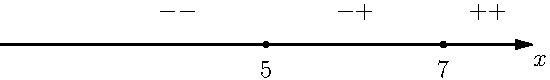
\includegraphics[scale =1]{7.pdf}\\
\end{center}
Разберем три случая.\\
\noindent
1) Пусть $x\leqslant5$. Тогда уравнение принимает вид:
\begin{center}
$-x+7-x+5=x-4 \Leftrightarrow -3x=-16\Leftrightarrow x=\dfrac{16}3.$\\
\end{center}
Так как $\frac{16}3>5$, то найденный корень $x=\frac{16}3$ -- не подходит под условие случая.\\[0.3cm]
\noindent
2) $5<x<7$\\
$-x+7+x-5=x-4 \Leftrightarrow x=6$\\
$5<6<7 \Rightarrow x=6 - \text{подходит.}$\\[0.3cm]
\noindent
3) $x\geqslant 7$\\
$x-7+x-5=x-4 \Leftrightarrow x=8$\\
$8\geqslant7 \Rightarrow x=8 - \text{подходит.}$\\

\Answer{\{6;8\}}
